\begin{figure}[H]
\centering
\subfigure{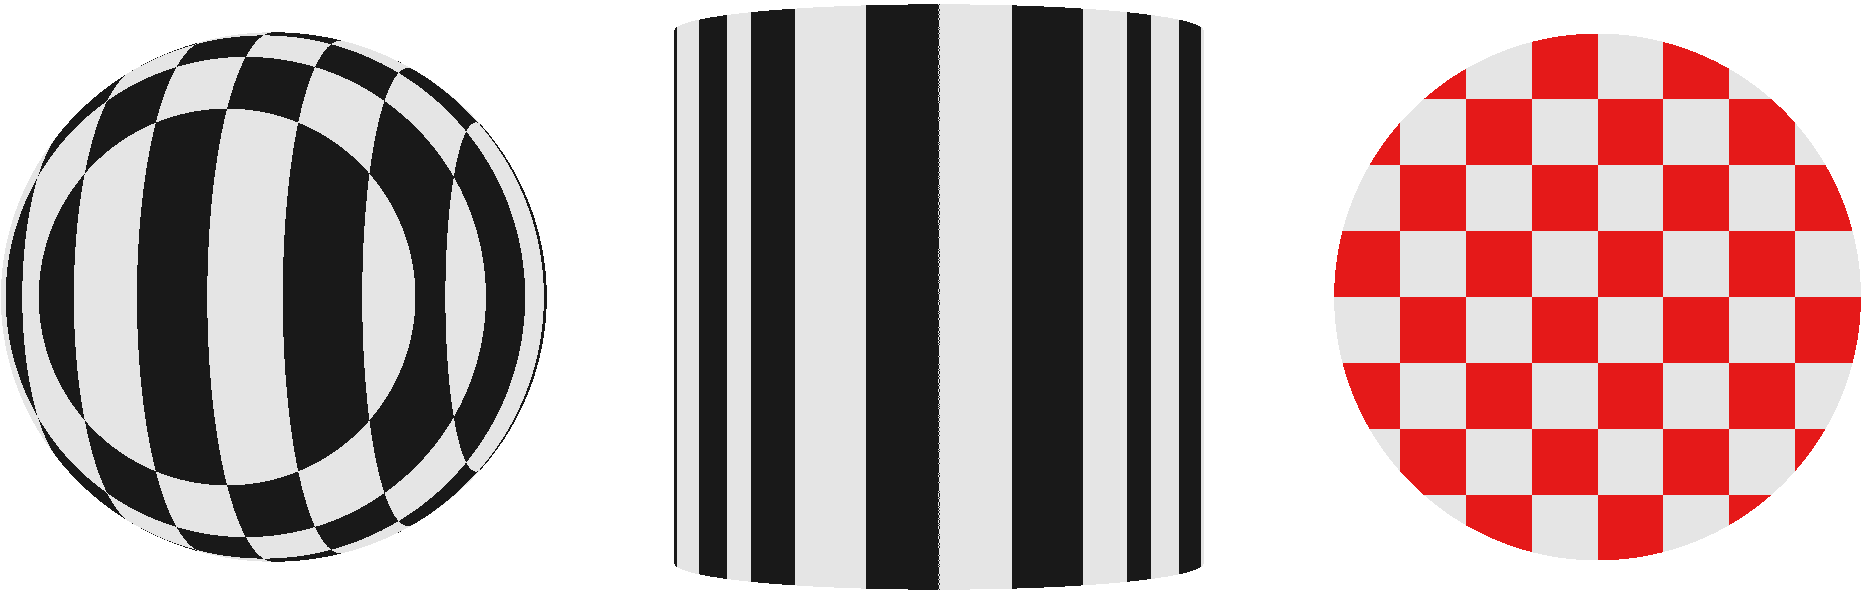
\includegraphics[width=0.55\textwidth]{chapters/ch3/img/texture_proj/planar.png}}
\subfigure{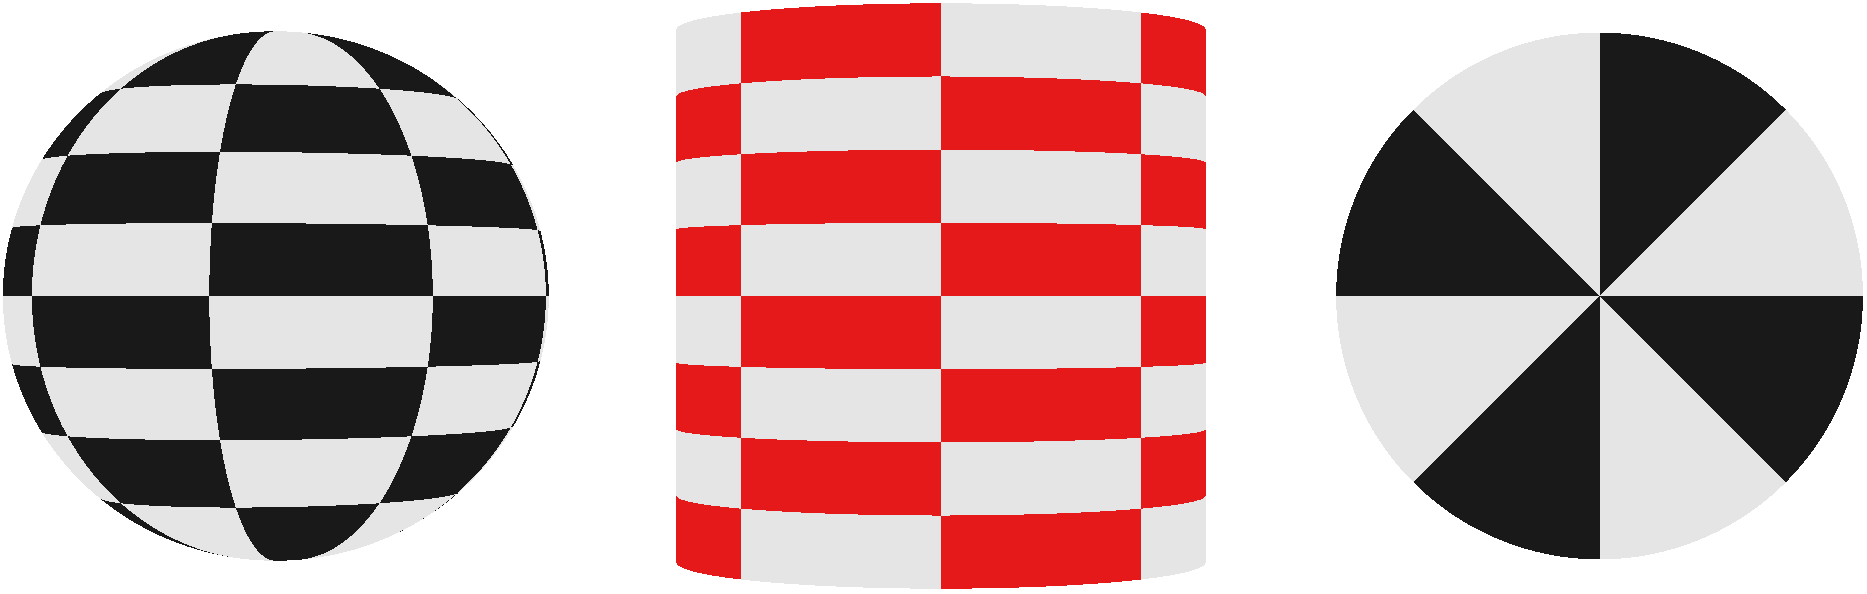
\includegraphics[width=0.55\textwidth]{chapters/ch3/img/texture_proj/cylindrical.png}}
\subfigure{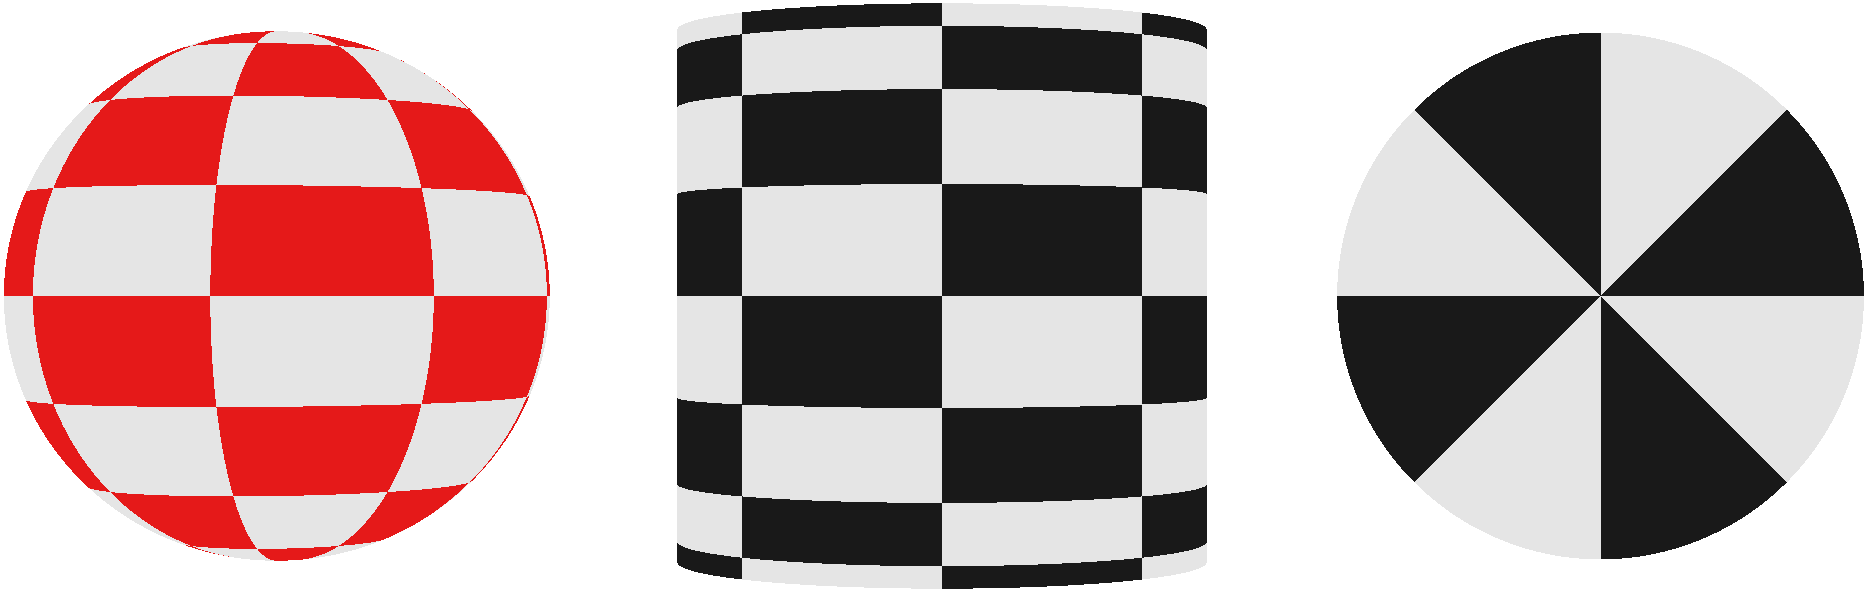
\includegraphics[width=0.55\textwidth]{chapters/ch3/img/texture_proj/spherical.png}}

\caption[Efekt nałożenia tekstury na różne typy obiektów w funkcji rodzaju zastosowanego mapowania]{Efekt nałożenia identycznej tekstury na różne typy obiektów w funkcji rodzaju zastosowanego mapowania. Od góry: mapowanie prostokątne, cylindryczne i sferyczne}
\label{ch3:img:texture_proj}
\end{figure}

